% -----------------------------------------------
% Template for FMA2016
% (based on ISMIR 2010 Template)
% -----------------------------------------------
%
% To compile run:
% pdflatex fma2016template.tex
% bibtex fma2016template
% pdflatex fma2016template.tex (probably twice)
%
% requires the newapa Bibtex style

\documentclass{article}
\usepackage[authoryear]{natbib}
\usepackage{fma2016}
\usepackage{amsmath}
\usepackage{graphicx}

% Title.
% ------
\title{PAPER TEMPLATE FOR FMA2016}

% Single address
% To use with only one author or several with the _same address_
% ---------------
%\oneauthor
% {Author}
% {Affiliation \\ {\tt {author}@fma.edu}}
%
\oneauthor
 {Author1, Author2}
 {Affiliation \\ {\tt \{author1,author2\}@fma.edu}}
%
% Two addresses
% --------------
%\twoauthors
%  {First author, Second Author} {Affiliation1 \\ {\tt author1@fma.edu, author2@afm.edu}}
%  {Third author} {Affiliation2 \\ {\tt author3@fma.edu}}
%
% Three addresses
% --------------
%\threeauthors
%  {First author} {Affiliation1 \\ {\tt author1@fma.edu}}
%  {Second author} {Affiliation2 \\ {\tt author2@fma.edu}}
%  {Third author} {Affiliation3 \\ {\tt author3@fma.edu}}


\begin{document}
%
\maketitle
%
\begin{abstract}
Only provide a short abstract at this place for a full paper. For an extended abstract, this abstract section should be removed.

The abstract should be placed at the top left column and should contain about 150-200 words. Font size is 9pt.
\end{abstract}
%
\section{Introduction}\label{sec:introduction}

This template includes all the information about format-ting manuscripts for the FMA proceedings. Please follow these guidelines to give the final proceedings a uniform look. If you have questions, please contact the workshop organizers. This template can be downloaded from the FMA website (http://fma-2016.sciencesconf.org).

\section{Page Size}\label{sec:page_size}

The proceedings will be printed on 
 \underline{portrait A4-size paper} \underline{(21.0cm x 29.7cm)}. 
All material on each page should fit within a rectangle of 17.2cm x 25.2cm, 
centered on the page, beginning 2.0cm 
from the top of the page and ending with 2.5cm from the bottom. 
The left and right margins should be 1.9cm. 
The text should be in two 8.2cm columns with a 0.8cm gutter. 
All text must be in a two-column format. 
Text must be fully justified.

\section{Typeset Text}\label{sec:typeset_text}

\subsection{Normal or Body Text}\label{subsec:body}

Please use a 10pt (point) Times font. Sans-serif or non-proportional fonts 
can be used only for special purposes, such as distinguishing source code text.

The first paragraph in each section should not be indented, but all other paragraphs should be.

\subsection{Title and Authors}

The title is 14pt Times, bold, caps, upper case, centered.
Authors' names are centered. 
The lead author's name is to be listed first (left-most), and the co-authors' names after. 
If the addresses for all authors are the same, include the address only once, centered. 
If the authors have different addresses, put the addresses, evenly spaced, under each authors' name.

\subsection{Page Numbering, Headers and Footers}

Do not include headers, footers or page numbers in your submission. 
These will be added when the publications are assembled.

\section{First Level Headings}

First level headings are in Times 10pt bold, 
centered with 1 line of space above the section head, and 1/2 space below it. 
For a section header immediately followed by a subsection header, the space should be merged.

\subsection{Second Level Headings}

Second level headings are in Times 10pt bold, flush left, 
with 1 line of space above the section head, and 1/2 space below it. 
The first letter of each significant word is capitalized.

\subsubsection{Third and Further Level Headings}

Third level headings are in Times 10pt italic, flush left, 
with 1/2 line of space above the section head, and 1/2 space below it. 
The first letter of each significant word is capitalized.

Using more than three levels of headings is highly discouraged.

\section{Footnotes and Figures}

\subsection{Footnotes}

Indicate footnotes with a number in the text.\footnote{This is a footnote.} 
Use 8pt type for footnotes. Place the footnotes at the bottom of the page on which they appear. 
Precede the footnote with a 0.5pt horizontal rule.

\begin{table}[h]
 \begin{center}
 \begin{tabular}{|l|l|}
  \hline
  Column A & Column B \\
  \hline
  Value 1  & Value 2 \\
  \hline
 \end{tabular}
\end{center}
 \caption{Table captions should be placed below the table.}
 \label{tab:example}
\end{table}

\begin{figure*}
 \centerline{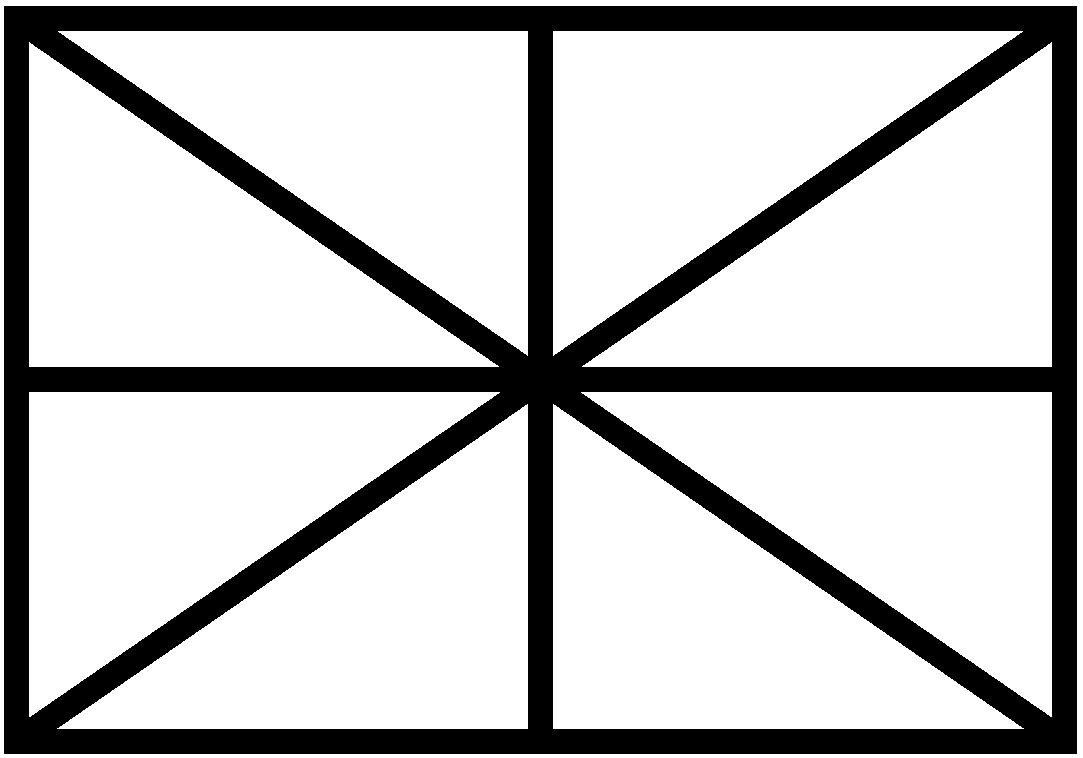
\includegraphics[width=7.49cm]{figure.png}\hskip1.5cm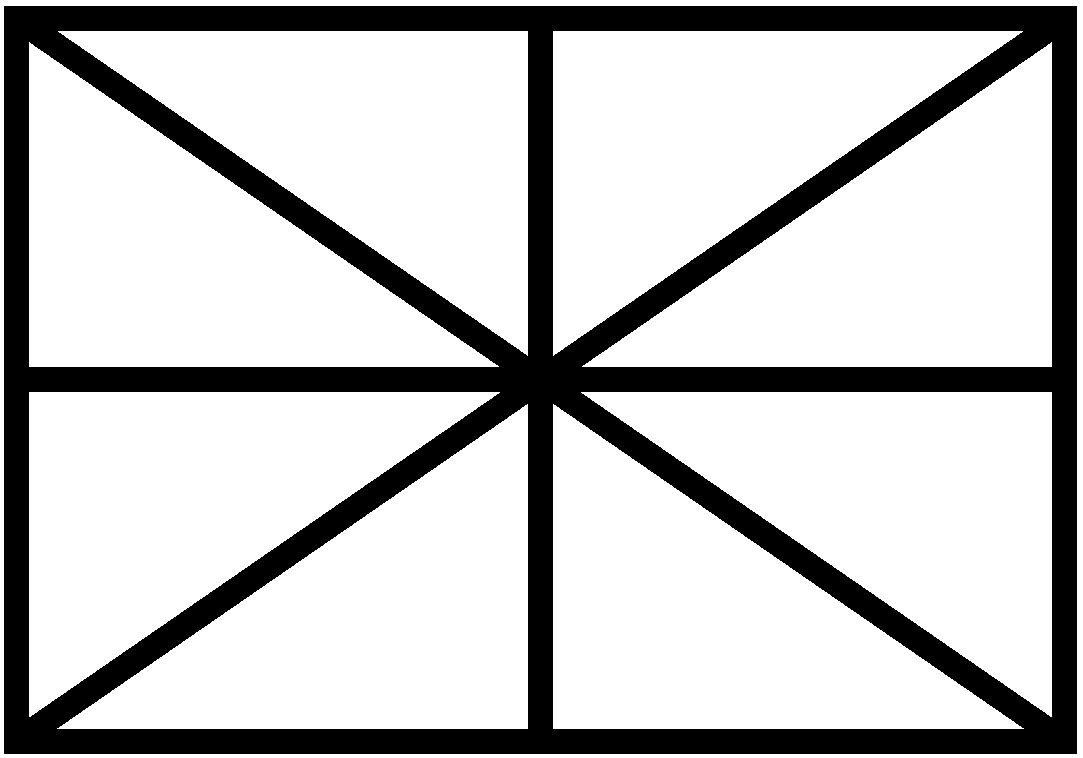
\includegraphics[width=7.49cm]{figure.png}}
 \caption{Figure captions should be placed below the figure.}
 \label{fig:example}
\end{figure*}


\subsection{Figures, Tables and Captions}

All artwork must be centered, neat, clean, and legible. 
All lines should be very dark for purposes of reproduction and art work should not be hand-drawn. 
It is recommended that all figures make sense in black-and-white form. 
Figure and table numbers and captions always appear below the figure. 
Leave 1 line space between the figure or table and the caption. 
Each figure or table is numbered consecutively. Captions should be Times 10pt. 
Place tables/figures in text as close to the reference as possible. 
References to tables and figures should be capitalized, for example: 
see \figref{fig:example} and \tabref{tab:example}. 
Figures and tables may extend across both columns to a maximum width of 17.2cm.


\section{Equations}

Equations should be placed on separated lines and numbered.
The number should be on the right side, in parentheses.

\begin{equation}
E=mc^{2}
\end{equation}

\section{Citations}

All bibliographical references should be listed at the end, 
inside a section named ``REFERENCES,'' numbered and in alphabetical order. 
Also, all references listed should be cited in the text. 
When referring to a document, use author-year (APA) style. E.g., ``\citet{Someone2010} raised the question whether\dots{}'', ``Previous research has shown that X always implies Y \citep{Smith2005,Author2000}.'', ``\citet{Writer2004} studied\dots''.

% Reference sheet at: ftp://ftp.tex.ac.uk/tex-archive/macros/latex/contrib/natbib/natnotes.pdf

\bibliography{fma2016bibliography}

\end{document}

